\documentclass[11pt, a4paper]{article}

% ─── Packages ────────────────────────────────────────────────────────────────
\usepackage[utf8]{inputenc}
\usepackage[T1]{fontenc}
\usepackage[margin=2.5cm]{geometry}
\usepackage{graphicx}
\usepackage{hyperref}
\usepackage{booktabs}       % nicer tables (\toprule, \midrule, \bottomrule)
\usepackage{float}          % [H] placement for figures and tables
\usepackage{xcolor}         % colors (used by listings)
\usepackage{listings}       % code listings
\hypersetup{colorlinks=true, linkcolor=black, citecolor=black, urlcolor=blue!70!black}

% ─── Code listing style ─────────────────────────────────────────────────────
\lstset{
    basicstyle=\ttfamily\small,
    breaklines=true,
    frame=single,
    numbers=left,
    numberstyle=\tiny\color{gray},
    xleftmargin=2em,
    framexleftmargin=1.5em
}
% Pro tip: for syntax highlighting, look into the 'minted' package.

% ─── Bibliography ────────────────────────────────────────────────────────────
\usepackage[style=numeric, backend=bibtex]{biblatex}
\addbibresource{references.bib}

% ─── Language (swap to lang/sk for Slovak) ───────────────────────────────────
\input{lang/en}

% ─── Student details ─────────────────────────────────────────────────────────
\newcommand{\StudentName}{Filip Kňažko, Markus Maslaňák}
\newcommand{\StudyGroup}{M. Petrík, Thursday 11:00}
\newcommand{\AssignmentNumber}{1}
\newcommand{\AssignmentTitle}{Database model design - music streaming service}
\newcommand{\AcademicYear}{2025/2026}

% =============================================================================
\begin{document}

% ─── Cover page ──────────────────────────────────────────────────────────────
\begin{titlepage}
    \centering

    \includegraphics[width=0.3\textwidth]{../assets/logo}

    \vspace{0.3cm}
    {\large \LabelUniversity}\\[2pt]
    {\large \LabelFaculty}

    \vspace{2.5cm}
    {\Huge\bfseries \LabelProtocol}

    \vspace{0.6cm}
    {\LARGE \LabelCode{} --- \LabelCourse}

    \vspace{0.4cm}
    {\Large \LabelAssignment{} \AssignmentNumber: \AssignmentTitle}

    \vfill

    \begin{tabular}{r l}
        \textbf{\LabelStudent:} & \StudentName  \\[4pt]
        \textbf{\LabelGroup:}   & \StudyGroup   \\[4pt]
        \textbf{\LabelYear:}    & \AcademicYear \\[4pt]
        \textbf{\LabelDate:}    & \today        \\
    \end{tabular}

    \vspace{1.5cm}
\end{titlepage}

% ─── Table of contents ───────────────────────────────────────────────────────
\renewcommand{\contentsname}{\LabelContents}
\tableofcontents
\newpage

% =============================================================================
% This document serves as both the assignment template and a quick guide
% to the LaTeX features you will need. Replace the content, keep the structure.
%
% Template source: https://github.com/FIIT-Databases/assignment-template
% =============================================================================

\section{Specification}
\label{sec:specification}

\subsection{System Overview}
The designed database system supports a music streaming app that allows users to listen to music, manage playlists, discover artists, and interact with other users. The system stores information about songs, albums, artists, genres, and user activity. It also tracks listening history and song ratings.\\
The purpose of this database is to provide a structured way to store and manage music-related data and enable efficient retrieval of information needed by the application.

\subsection{Main actors}
\paragraph{Music listeners:} Regular users of the platform who listen to music, create playlists, follow artists, and interact with other users.
\paragraph{Artists:} Musicians or music creators whose songs and albums are published in the system. They may release albums, songs, and participate in concerts.
\paragraph{Administrators:} Administrators may manage the music catalog, verify artist profiles, and other systems to maintain the platform.

\subsection{Main entities}
\paragraph{User:} Represents a registered user of the platform. Provides basic information about the user.
\paragraph{Song:} Represents an individual music track. Each song belongs to an album and can be associated with multiple artists and genres.
\paragraph{Playlist:} Represents a collection of songs created by users. Users can use them to sort their favorite songs.
\paragraph{ListeningHistory:} Records every instance of a user listening to a song. It is useful for tracking activity, generating recommendations, and analyzing popularity.

\subsection{Rules and restrictions}
\begin{itemize}
    \item Each user can have only one role: user, artist, or admin.
    \item Adding or removing songs can only be done by admins and artists if it is their song.
    \item Each song must correspond to one album. If it is a single it has album with only that song.
    \item Each song must have at least one artist.
    \item Each song must be set to at least one genre.
    \item Songs rating is limited to range 1 to 5 included.
\end{itemize}


\newpage
\section{User scenarios}
\label{sec:scenarios}

\subsection{Scenario 1: Creating a personal playlist and adding a song}

\textbf{Description:}\\
A user creates a new personal playlist and adds a song of their choice to the playlist.

\paragraph{Prerequisites:}
\begin{itemize}
    \item A user must be logged in.
\end{itemize}

\paragraph{Main flow:}
\begin{enumerate}
    \item The user navigates to the "Your library" section and selects the "Create new playlist" option.
    \item The User enters a title (e.g. "Gym mix") and confirms.
    \item The User searches for a specific song using the search bar.
    \item The User selects the "Add to playlist" option from the song's context menu and chooses the newly created playlist.
    \item The system confirms the addition and refreshes the playlist view.
\end{enumerate}

\paragraph{Data layer:}
\begin{enumerate}
    \item Take the user ID from the session.
    \item INSERT into the \texttt{Playlist} table to create the new playlist (the insertion may be unsuccessful).
    \item INSERT into the \texttt{UserToPlaylist} junction table.
    \item SELECT from the \texttt{Song} table where \texttt{isPublic = True}.
    \item INSERT into the \texttt{SongToPlaylist} table.
\end{enumerate}

\paragraph{Alternative flow:}
\begin{itemize}
    \item \textbf{A1:} If the user does not provide a title, the system defaults to "New Playlist \#X".
    \item \textbf{A2:} If a playlist with this title already exists, the system prompts the user to choose a different one.
    \item \textbf{A3:} If the song the user searches for is not made public, the system shows no search results and has to search for a different song.
\end{itemize}

\subsection{Scenario 2: Artist Releasing a New Album}

\textbf{Description:}\\
A verified artist uploads a collection of tracks to publish their new album.

\paragraph{Prerequisites:}
\begin{itemize}
    \item A user with an \texttt{artist} role must be logged in.
    \item A user with an \texttt{administrator} role must be logged in.
\end{itemize}

\paragraph{Main flow:}
\begin{enumerate}
    \item The artist opens the "Creator Studio" and selects "Upload New Album".
    \item The artist fills in the album name, release date, and other metadata.
    \item The artist uploads the individual songs for the album.
    \item The artist clicks "Publish album".
    \item The administrator searches for unverified albums and selects one for verification.
    \item The administrator verifies each song from the album and sets every verified song to public, making it available to all users.
\end{enumerate}

\paragraph{Data layer:}
\begin{enumerate}
    \item The Artist's user ID is collected from their session.
    \item INSERT into the \texttt{Album} table.
    \item INSERT into the \texttt{AlbumToArtist} junction table.
    \item INSERT into the \texttt{Song} table.
    \item SELECT from the
\end{enumerate}

\begin{itemize}
    \item \textbf{Entity creation:} A record is created in the \texttt{Album} table.
    \item \textbf{Batch insertion:} Multiple records are inserted into the \texttt{Song} table, each using the new \texttt{Album.id} as a foreign key.
    \item \textbf{Record Update:} An insertion occurs in the \texttt{AlbumToArtist} junction table linking the \texttt{Album.id} to the \texttt{Artist.id}.
\end{itemize}

\paragraph{Alternative flows:}
\begin{itemize}
    \item \textbf{A1:} If any song file fails validation (e.g., corrupted file, quality too low), the system stops publication and notifies the artist.
    \item \textbf{A2:} If the release date is set in the future, the album status is set to "Scheduled" instead of "Live", making it visible but unplayable to all users.
\end{itemize}

\paragraph{Diagram(s):}

\subsection{Scenario 3: Displaying listening statistics for a selected period}

\textbf{Description:}
A user requests statistics of their activity (e.g., top artists, total minutes) for a specific time frame (past week, month, or year).

\paragraph{Main flow:}
\begin{enumerate}
    \item The User visits their "Profile" and selects "My Stats".
    \item The User selects a time frame (e.g., "Last month") and clicks "Generate Report".
    \item The system processes the history and displays the top 5 artists and total listening time for the selected time frame.
\end{enumerate}

\paragraph{Data layer:}
\begin{itemize}
    \item \textbf{Filtering:} The system queries \texttt{ListeningHistory} table, filtering by the \texttt{listenedAt} attribute.
    \item \textbf{Aggregation:} Aggregation functions \texttt{SUM} and \texttt{COUNT} are used to process the filtered history to produce the final statistics that will be shown to the user.
\end{itemize}

\paragraph{Alternative flow:}
\begin{itemize}
    \item \textbf{A1:} If there is no data for the selected period, the system displays a "No activity found" message and suggests a broader time frame.
\end{itemize}

\paragraph{Diagram(s):}

\subsection{Scenario 4: User rating a song}

\textbf{Description:}\\
A user provides a star rating (1-5) for the selected song, which causes the recalculation of the average rating displayed to all users.

\paragraph{Main flow:}
\begin{enumerate}
    \item The user clicks the "Rate" button on the app's player interface.
    \item The user selects a value from 1 to 5 stars.
    \item The system records the rating, calculates the new average for the track, and updates the displayed rating.
\end{enumerate}

\paragraph{Data layer:}
\begin{itemize}
    \item \textbf{Record creation:} A new record is inserted into the \texttt{UserSongRating} table (or updated if the user has already rated it), containing \texttt{User.id}, \texttt{Song.id}, \texttt{rating}.
    \item \textbf{Aggregation:} The system performs the \texttt{AVG} aggregate function on the \texttt{UserSongRating} table filtered by the specific \texttt{songId} and then updates the average stored in the \texttt{Song} table.
\end{itemize}

\paragraph{Alternative flows:}
\begin{itemize}
    \item \textbf{A1:} If the user tries to rate a song they have not listened to, the system prompts them to listen to it first.
\end{itemize}

\paragraph{Diagram(s):}
lorem ipsum
\newline

We compared a few approaches before settling on the current structure.
Table~\ref{tab:comparison} summarizes our options.

% ── Tables ───────────────────────────────────────────────────────────────────
% Use \begin{table}[H] to place the table exactly here.
% Label it with \label{} and reference it with Table~\ref{}.

\begin{table}[H]
    \centering
    \caption{Comparison of template approaches}
    \label{tab:comparison}
    \begin{tabular}{l c c c}
        \toprule
        \textbf{Approach}  & \textbf{Easy to edit} & \textbf{Bilingual} & \textbf{Compiles anywhere} \\
        \midrule
        Word document       & yes                   & manual             & n/a  \\
        Markdown + Pandoc   & yes                   & no                 & maybe \\
        \LaTeX{} template   & yes                   & yes                & yes  \\
        \bottomrule
    \end{tabular}
\end{table}

We chose \LaTeX{} because it handles structured documents, citations,
and cross-references well --- things that matter when writing technical
reports\footnote{It also looks way better than a Word document. But we are
biased.}. Unrelated: the wood frog can survive being frozen solid for months ---
its heart stops, it stops breathing, and in spring it just thaws and hops away.
We found this less stressful than debugging \LaTeX{} table alignment.


\newpage
\section{Implementation}
\label{sec:implementation}

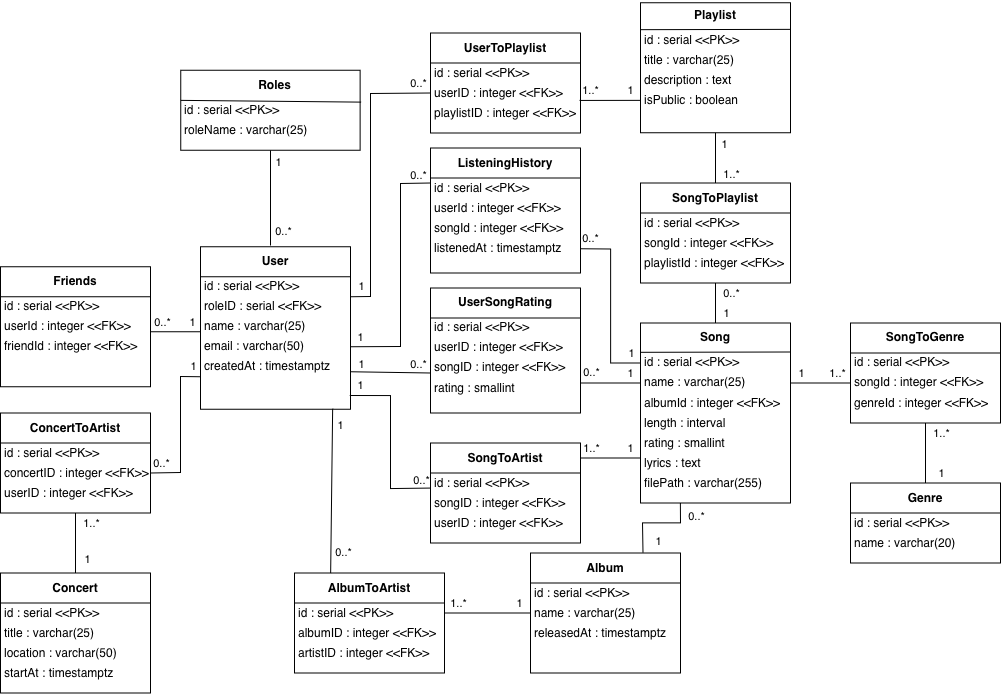
\includegraphics[width=1.0\textwidth]{../assets/DBS}
Figure~\ref{fig:diagram1}

\subsection{Table Relationships and Cardinalities}

\begin{itemize}
    \item \textbf{User -- Role (M:1)} \\
    A user must have exactly one role, and a role can be assigned to multiple users.
    \item \textbf{User -- Friends (1:N)} \\ 
    A user can have zero or more friends.
    \item \textbf{User -- Playlist (M:N)} \\
    A user can collaborate on zero or more playlists, and a playlist must have at least one collaborator.
    \item \textbf{User -- Song (user creating song) (M:N)} \\
    An artist can create zero or more songs, and a song can be created by at least one artist.
    \item \textbf{User -- Song (listening history) (M:N)} \\
    A user may have listened to zero or more songs, and a song may have been listened to by zero or more users.
    \item \textbf{User -- Song (song rating) (1:N)} \\
    A user can give a rating to zero or more songs, and a song may have been rated by zero or more users.
    \item \textbf{Song -- Playlist (M:N)} \\
    A song can be in zero or more playlists, and a playlist can have zero or more songs.
    \item \textbf{Song -- Genre (M:N)} \\
    A song must belong to at least one genre, and a genre can have zero or more songs.
    \item \textbf{User -- Album (M:N)} \\
    An artist can create zero or more albums, and an album can be created by many artists.
    \item \textbf{Song -- Album (1:N)} \\
    A song must belong to a single album, and an album can have zero or more songs.
    \item \textbf{User -- Concert (M:N)} \\
    An artist can have zero or more concerts scheduled, and a concert must have one or more artists.
\end{itemize}

\subsection{Table descriptions}

All tables except \texttt{User} are \texttt{ON DELETE RESTRICT} (set to null). \texttt{User} table is \texttt{ON DELETE CASCADE} (set to null).

\paragraph{User}~\\
The User table stores information about all registered users. Users can create playlists, follow artists and playlists, rate songs, listen to songs, and connect with other users.
~\\\textbf{Attributes:}
\begin{itemize}
    \item \textbf{id:} unique identifier of the user (PRIMARY KEY).
    \item \textbf{role:} enum identifying the user's role. It can be: user, artist, admin.
    \item \textbf{name:} username displayed in the application.
    \item \textbf{email:} user's email address.
    \item \textbf{createdAt:} timestamp indicating when the user account was created.
\end{itemize}

\paragraph{Friends}~\\
The Friends table represents friendship relationships between users.
~\\\textbf{Attributes:}
\begin{itemize}
    \item \textbf{id:} unique identifier of the relationship (PRIMARY KEY).
    \item \textbf{userId:} identifier of the user (FOREIGN KEY)
    \item \textbf{friendId:} identifier of the friend (also a user) (FOREIGN KEY)
\end{itemize}

\paragraph{Playlist}~\\
The Playlist table stores playlists created in the system. Playlists can contain multiple songs.
~\\\textbf{Attributes:}
\begin{itemize}
    \item \textbf{id:} unique identifier of the playlist (PRIMARY KEY).
    \item \textbf{title:} playlist title
    \item \textbf{description:} description of the playlist
    \item \textbf{isPublic:} indicates whether the playlist is publicly visible to other users apart from the creator.
\end{itemize}

\paragraph{UserToPlaylist}~\\
The UserToPlaylist table represents the relationship between users and playlists they own.
~\\\textbf{Attributes:}
\begin{itemize}
    \item \textbf{id:} unique identifier of the relationship (PRIMARY KEY).
    \item \textbf{userId:} identifier of the user who owns the playlist (FOREIGN KEY)
    \item \textbf{playlistId:} identifier of the playlist (FOREIGN KEY)
\end{itemize}

\paragraph{ListeningHistory}~\\
The ListeningHistory table records all song playback events. This table is useful for recommendations, statistics, and tracking users activity.
~\\\textbf{Attributes:}
\begin{itemize}
    \item \textbf{id:} unique identifier of the record (PRIMARY KEY).
    \item \textbf{userId:} identifier of the user who listened to the song (FOREIGN KEY)
    \item \textbf{songId:} identifier of the song (FOREIGN KEY)
    \item \textbf{listenedAt:} timestamp when the song was played
\end{itemize}

\paragraph{SongToPlaylist}~\\
The SongToPlaylist table represents the many-to-many relationship between songs and playlists.
~\\\textbf{Attributes:}
\begin{itemize}
    \item \textbf{id:} unique identifier of the relationship (PRIMARY KEY).
    \item \textbf{songId:} identifier of the song (FOREIGN KEY)
    \item \textbf{playlistId:} identifier of the playlist (FOREIGN KEY)
\end{itemize}

\paragraph{UserSongRating}~\\
The UserSongRating table stores ratings given by users to songs. This allows users to evaluate songs and helps the system compute song popularity.
~\\\textbf{Attributes:}
\begin{itemize}
    \item \textbf{id:} unique identifier of the record (PRIMARY KEY).
    \item \textbf{userId:} identifier of the user who rated the song (FOREIGN KEY)
    \item \textbf{songId:} identifier of the rated song (FOREIGN KEY)
    \item \textbf{rating:} numeric rating value (CHECK(rating >= 1 AND rating <= 5))
\end{itemize}

\paragraph{Song}~\\
The Song table stores information about individual songs. Songs can belong to albums, playlists, genres, and artists. Song's rating is calculated as average from \texttt{UserSongRating} table.
~\\\textbf{Attributes:}
\begin{itemize}
    \item \textbf{id:} unique identifier of the song (PRIMARY KEY).
    \item \textbf{name:} song title
    \item \textbf{albumId:} identifier of the album containing the song (FOREIGN KEY, NOT NULL)
    \item \textbf{length:} duration of the song
    \item \textbf{rating:} rating of the song, calculated as average from \texttt{UserSongRating} table.
    \item \textbf{lyrics:} song lyrics
    \item \textbf{filePath:} path where the audio file is located
\end{itemize}

\paragraph{Genre}~\\
The Genre table stores music genre categories.
~\\\textbf{Attributes:}
\begin{itemize}
    \item \textbf{id:} unique identifier of the record (PRIMARY KEY).
    \item \textbf{name:} name of the genre
\end{itemize}

\paragraph{SongToGenre}~\\
The SongToGenre table represents the many-to-many relationship between songs and genres.
~\\\textbf{Attributes:}
\begin{itemize}
    \item \textbf{id:} unique identifier of the relationship (PRIMARY KEY).
    \item \textbf{songId:} identifier of the song (FOREIGN KEY)
    \item \textbf{genreId:} identifier of the genre (FOREIGN KEY)
\end{itemize}

\paragraph{Album}~\\
The Album table stores information about music albums. Albums group multiple songs together. One song can belong to only one album.
~\\\textbf{Attributes:}
\begin{itemize}
    \item \textbf{id:} unique identifier of the album (PRIMARY KEY).
    \item \textbf{songId:} album title
    \item \textbf{genreId:} timestamp indicating album release date
\end{itemize}

\paragraph{AlbumToArtist}~\\
The AlbumToArtist table represents the many-to-many relationship between albums and artists. This allows multiple artists to collaborate on the same album.
~\\\textbf{Attributes:}
\begin{itemize}
    \item \textbf{id:} unique identifier of the relationship (PRIMARY KEY).
    \item \textbf{albumId:} identifier of the album (FOREIGN KEY)
    \item \textbf{artistId:} identifier of the artist (FOREIGN KEY)
\end{itemize}

\paragraph{Concert}~\\
The Concert table stores information about concerts. Concerts represent live performances. Multiple artists can perform at a single concert.
~\\\textbf{Attributes:}
\begin{itemize}
    \item \textbf{id:} unique identifier of the concert (PRIMARY KEY).
    \item \textbf{title:} concert title
    \item \textbf{location:} concert location where it is happening
    \item \textbf{startAt:} timestamp of the concert start
\end{itemize}

\paragraph{ConcertToArtist}~\\
The ConcertToArtist table represents the many-to-many relationship between concerts and artists. This allows multiple artists to perform at a single concert.
~\\\textbf{Attributes:}
\begin{itemize}
    \item \textbf{id:} unique identifier of the relationship (PRIMARY KEY).
    \item \textbf{concertId:} identifier of the album (FOREIGN KEY)
    \item \textbf{artistId:} identifier of the artist (FOREIGN KEY)
\end{itemize}


\paragraph{----- TO BE DELETED -----}
The template lives in a simple directory structure with localization files
separated from the main document. Switching language requires changing one
line:

% ── Code listings ────────────────────────────────────────────────────────────
% Use lstlisting for short code snippets.

\begin{lstlisting}[language=TeX, caption={Switching language in the preamble}]
% English
\input{lang/en}

% Slovak
\input{lang/sk}
\end{lstlisting}

For SQL or other languages, change the \texttt{language} parameter:

\begin{lstlisting}[language=SQL, caption={Example SQL query}]
SELECT s.name, COUNT(*) AS submission_count
FROM students s
JOIN submissions sub ON s.id = sub.student_id
GROUP BY s.name
ORDER BY submission_count DESC;
\end{lstlisting}

% ── Inline code ──────────────────────────────────────────────────────────────
% Use \texttt{} for inline code: \texttt{SELECT * FROM ...}

References to tables, figures, and sections are automatic. For example,
this is Section~\ref{sec:implementation}, the comparison is in
Table~\ref{tab:comparison}, and the faculty logo is shown in
Figure~\ref{fig:logo} in Attachment~\ref{sec:attachment-a1}.
If you add or reorder content, the numbers update on the next build.

% ── Citations ────────────────────────────────────────────────────────────────
% Add entries to references.bib, then cite them with \cite{key}.
% The bibliography at the end is generated automatically.

The database fundamentals referenced throughout the course are covered
in \cite{elmasri2016}. For PostgreSQL-specific syntax, see
\cite{postgresql-docs}.


\newpage
\section{Challenges}
\label{sec:challenges}

The main challenge was keeping the template simple enough that a student
seeing \LaTeX{} for the first time would not immediately close the file.
We solved this by limiting the preamble to essential packages and
putting all examples in one place --- this document.

We also learned that BibTeX interprets \texttt{@} signs in comments as
entry types, which caused confusing errors. Small things like this are
easy to fix once you know about them, but hard to debug the first time\footnote{A
group of frogs is called an ``army.'' A group of students debugging BibTeX at
2\,AM is called ``Tuesday.''}.


\newpage
\section{Conclusion}
\label{sec:conclusion}

The template meets the requirements from Section~\ref{sec:specification}.
It compiles with a standard \LaTeX{} distribution, supports two
languages, and provides working examples of every feature students
are likely to need.

For anything not covered here, the Overleaf documentation
\cite{overleaf-docs} is an excellent reference.

% ─── Bibliography ────────────────────────────────────────────────────────────
\printbibliography

% ─── Attachments ─────────────────────────────────────────────────────────────
\newpage
\appendix

\section{Sample figures}
\label{sec:attachment-a1}

% ── Figures ──────────────────────────────────────────────────────────────────
% Use \begin{figure}[H] to place the figure exactly here.
% Label it with \label{} and reference it with Figure~\ref{}.
% Keep images in the assets/ directory.

\begin{figure}[H]
    \centering
    \includegraphics[width=0.25\textwidth]{../assets/logo}
    \caption{Faculty logo used on the cover page}
    \label{fig:logo}
\end{figure}

\begin{figure}[H]
    \centering
    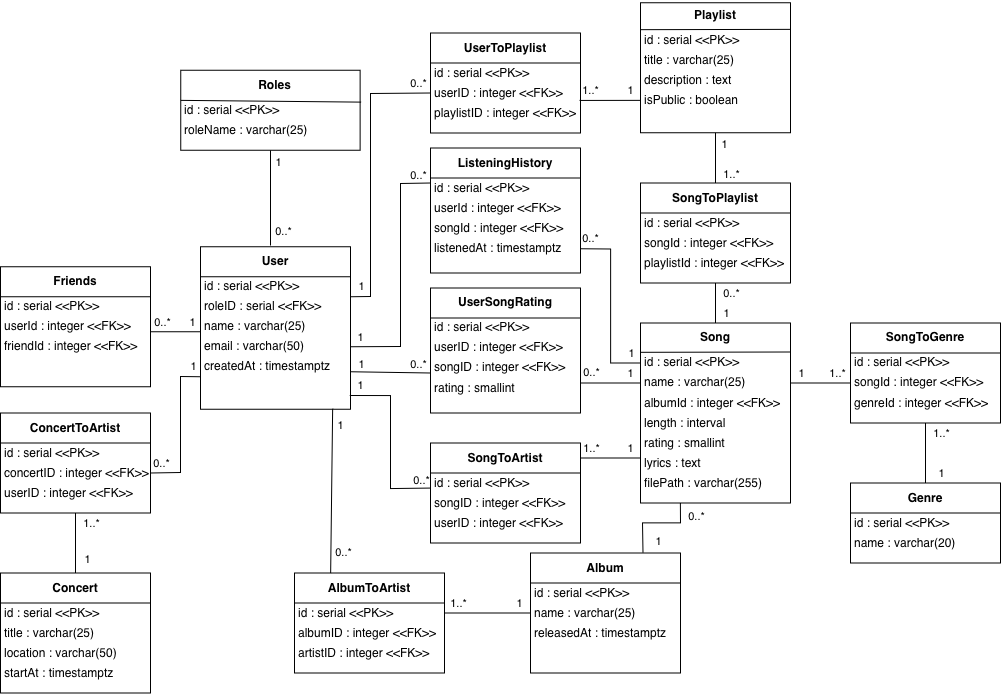
\includegraphics[width=1\linewidth]{../assets/DBS.png}
    \caption{Physical data model of our database}
    \label{fig:diagram1}
\end{figure}

Place your diagrams, screenshots, and other supporting images in this
section. Reference them from the main text using
\texttt{Figure\~{}\textbackslash ref\{fig:logo\}}.

Some frogs can absorb water through a patch of skin on their belly called a
``drinking patch'' --- they literally sit in puddles to hydrate. This has
nothing to do with databases but is objectively more interesting than
anything on this page.

% You can control the image size with the width parameter:
%   width=0.5\textwidth   ... half the page width
%   width=5cm             ... exact size
%   scale=0.8             ... 80% of original

% To add more figures, copy the block above and change the file path,
% caption, and label.

\end{document}